% P5 manuscript — target: Journal of Cheminformatics (Springer Nature)
% Draft v1 — Aug 2026. Initial submission format-flexible.
\documentclass[11pt,a4paper]{article}

\usepackage[margin=1in]{geometry}
\usepackage{amsmath,amssymb}
\usepackage{authblk}
\usepackage{booktabs}
\usepackage{graphicx}
\graphicspath{{../results/figures/}}
\usepackage{hyperref}
\usepackage{microtype}
\usepackage[numbers,sort&compress]{natbib}
\usepackage{xcolor}

\title{\textbf{Larger models, unchanged verdict: a controlled benchmark of graph neural networks and transformers against ECFP4 fingerprints for antimalarial natural-product activity prediction}}

\author[1]{Myke Vital Sao Temgoua\thanks{Corresponding author: myke-vital.sao@facsciences-uy1.cm}}
\author[1]{Jean-Pierre Tchapet Njafa}
\author[1]{Serge Guy Nana Engo}
\author[2]{Penabei Samafou}
\author[3]{Wilfred Fon Mbacham}

\affil[1]{Department of Physics, Faculty of Science, University of Yaound\'e I, P.O. Box 812, Yaound\'e, Cameroon}
\affil[2]{Department of Medical Imaging and Radiation Sciences, Universit\'e de Sherbrooke, Sherbrooke, QC, Canada}
\affil[3]{Department of Biochemistry, Faculty of Science, University of Yaound\'e I, P.O. Box 812, Yaound\'e, Cameroon}

\date{\today}

\begin{document}

\maketitle

\begin{abstract}
The growing availability of pretrained molecular foundation models and large sequence transformers has fuelled the expectation that ``larger models'' should systematically outperform compact cheminformatics models on molecular property prediction. We test this assumption on a curated panel of \textbf{19,836 African antimalarial natural products} assembled from the eOS80CH screening collection, under both a random and a Bemis--Murcko scaffold five-fold cross-validation (25 fold--seed replicates). We compare a random-forest baseline on ECFP4 fingerprints against a graph isomorphism network (GIN), two topological fusion variants (GIN--TFP and GIN--TNE built on persistent-homology and tensor-network descriptors), and a fine-tuned ChemBERTa sequence transformer. Under the scaffold split -- the practically relevant out-of-distribution setting -- \textbf{ECFP4--RF achieves the highest ROC AUC (0.8300), followed by GIN--TFP (0.8138), GIN--TNE (0.8090), GIN (0.8047), and ChemBERTa (0.7867)}. No GNN or transformer arm significantly outperforms the fingerprint baseline; ChemBERTa is significantly worse ($\Delta = -0.043$, paired $t$, $p < 0.0001$). We further show that a leak-aware analysis is essential: naive per-fold reuse of pretrained weights inflates transformer AUCs by up to 0.15, an artifact we document and correct. Finally, an attribution analysis of the fusion head reveals that \textbf{persistent-image dimensions of the topological fingerprints carry the majority of the predictive signal}, providing an interpretable link to the underlying molecular geometry. Our results mirror and extend the recent ``Do Larger Models Really Win?'' benchmark on a clinically motivated natural-product panel, and support the emerging view that representation--task alignment, not model scale, governs predictive performance in small-molecule activity prediction. Code, frozen splits, and trained checkpoints are released.
\end{abstract}

\noindent\textbf{Keywords:} graph neural networks; molecular fingerprints; antimalarial natural products; scaffold split; benchmark; interpretability; persistent homology

\section{Introduction}

Malaria remains a leading infectious disease burden in sub-Saharan Africa, with 247\,million cases and 619{,}000 deaths in 2023 alone \citep{who2024malariareport}. Control is increasingly threatened by the emergence of artemisinin-resistant \emph{Plasmodium falciparum} strains in Southeast Asia and Africa \citep{ariyey2014,ashley2018}, prompting an urgent, WHO-endorsed need for new scaffolds that remain active against drug-resistant parasites. African natural products (NPs) constitute a rich, historically validated source of such scaffolds \citep{anpdb_2026,value_addition_african_np_2025}; the antimalarial panel studied here descends from a screening campaign seeded on 396 African NP and 454 synthetic-drug scaffolds \citep{temgoua2026antimalarial}. Computational screening of NP libraries promises to accelerate hit identification in this resistance-driven search, yet the cheminformatics tools chosen for this task strongly condition the outcome. In recent years, a ``scale-centric'' narrative has emerged in molecular machine learning: pretrained molecular foundation models and sequence transformers are expected to supersede compact, task-trained cheminformatics models \citep{mol_tdl_2026,tn_efficient_2026}.

This narrative is increasingly challenged by rigorous, controlled benchmarks. In a 156-comparison benchmark across 26 endpoints, Guo and Ding found that classical machine learning on fingerprints wins 47.4\% of task--metric entries, ahead of pretrained sequence models (28.8\%) and GNNs (21.8\%), with the classical advantage largest under random splits and shrinking, but not vanishing, under scaffold-separated protocols \citep{guo_ding_2026}. An independent comparison of 25 pretrained embedding models across 25 datasets found that \emph{almost no neural embedding statistically improves over the ECFP fingerprint baseline} \citep{benchmark_pretrained_2025}. And for natural products specifically, a 20-fingerprint benchmark over 100,000+ NPs showed that no single encoding dominates, and that ECFP is frequently matched or exceeded by alternative fingerprints on NP bioactivity tasks \citep{boldini2024}.

Three gaps remain, which motivate the present study. \emph{First}, existing scale-benchmarks are dominated by drug-like libraries (ADMET, Tox21); the conclusion ``compact models suffice'' has not been controlled on a dedicated antimalarial NP panel, whose structural diversity (higher fraction of sp$^3$ carbons, multiple stereocenters) stresses fingerprint-based representations. \emph{Second}, although topological descriptors (persistent homology) and tensor-network embeddings have been advocated as richer representations \citep{tda_review_2025,topology_molecular_representations_2025,tn_efficient_2026}, their value has rarely been tested \emph{inside} a modern GNN fusion architecture under a scaffold split. \emph{Third}, published transformer benchmarks rarely audit for a subtle but serious failure mode: cross-fold leakage of pretrained weights when a single model instance is fine-tuned on successive folds without reset. We encountered exactly this artifact, quantify its inflation, and publish the corrected protocol.

We therefore ask a deliberately conservative question: \emph{On a controlled antimalarial NP panel, do GNNs and a pretrained sequence transformer outperform a random forest on ECFP4, under both random and scaffold splits?} We find they do not. The contribution of this work is threefold: (i) a controlled, leak-audited, reproducible benchmark of GNNs and a transformer on 19,836 antimalarial NPs, under random and scaffold splits; (ii) a documentation and correction of a cross-fold weight-leakage artifact in transformer fine-tuning, with honest post-fix results; (iii) an interpretability analysis showing that persistent-image topological features dominate the fusion model's predictive signal, providing a link between learned representations and molecular geometry that remains actionable even when predictive gains are absent.

\section{Results}

\subsection{Reproducibility of the baseline: same panel, same fingerprints, same verdict}

As a sanity gate, we reproduced the ECFP4--RF baseline from the companion quantum-representation study \citep{temgoua2027quantum} on the identical frozen panel. Under the random split we obtain $0.9433 \pm 0.0002$ (per-seed range 0.9428--0.9437), against the reference value of $0.9475 \pm 0.0045$; the $0.004$ gap is within the reported uncertainty and reflects a different random CV draw of the same molecules. This reproducibility gate establishes that our benchmark shares the same chemical panel and feature pipeline as prior work, so that cross-project comparisons are valid.

\subsection{H1: no GNN or topological fusion beats ECFP4 under scaffold}

\begin{table}[t]
\centering
\caption{Mean test ROC AUC $\pm$ std across 25 fold--seed replicates, random and scaffold splits. Paired $t$-tests (5 per-seed means) vs.\ ECFP4--RF under scaffold.}
\label{tab:h1}
\begin{tabular}{lccc}
\toprule
Model & Random & Scaffold & $\Delta$ vs.\ ECFP4 (scaffold, $p$) \\
\midrule
ECFP4--RF (baseline) & 0.9433 $\pm$ 0.0002 & \textbf{0.8300} $\pm$ 0.0023 & --- \\
GIN & 0.9098 $\pm$ 0.0067 & 0.8047 $\pm$ 0.0395 & $-0.025$ ($p=0.051$, ns) \\
GIN--TFP (topological fusion) & --- & 0.8138 $\pm$ 0.0352 & $-0.016$ ($p=0.081$, ns) \\
GIN--TNE (tensor fusion) & --- & 0.8090 $\pm$ 0.0378 & $-0.023$ ($p=0.015$*) \\
ChemBERTa & 0.9121 $\pm$ 0.0047 & 0.7867 $\pm$ 0.0338 & $-0.043$ ($p<0.0001$***) \\
\bottomrule
\end{tabular}
\end{table}

Table~\ref{tab:h1} reports mean test ROC AUC across 25 fold--seed replicates for each model, under both splits. Under the scaffold split, the fingerprint baseline reaches \textbf{0.8300}. The best GNN arm, the topological fusion GIN--TFP, reaches 0.8138 ($\Delta = -0.016$, paired $t$, $p = 0.081$, ns); GIN--TNE reaches 0.8090 ($\Delta = -0.023$, $p = 0.015$, significantly \emph{worse}); plain GIN reaches 0.8047 ($\Delta = -0.025$, $p = 0.051$, ns). Under the random split, GIN reaches 0.9098, still 0.034 below ECFP4--RF (0.9433). \textbf{No graph-based arm outperforms the fingerprint baseline under either split.}

This is not an implementation artifact: the GNN training is standard (AdamW, patience-early stopping, best-val checkpointing, 25 replicates), and the sanity gate above verifies the shared pipeline. Rather, it reproduces, on an antimalarial NP panel, the pattern reported across ADMET/Tox21 endpoints \citep{guo_ding_2026} and across 25 pretrained-embedding benchmarks \citep{benchmark_pretrained_2025}: on datasets of a few thousand labelled molecules, local substructure encodings captured by ECFP4 and exploited by tree ensembles are more data-efficient than learned graph representations.

\subsection{H2: the sequence transformer is honest, and loses}

ChemBERTa, fine-tuned with per-fold weight reset (see Methods), reaches \textbf{0.7867 $\pm$ 0.0338} under the scaffold split (25 replicates, fold range 0.724--0.836). Against the 0.8300 fingerprint baseline this is a significant deficit ($\Delta = -0.043$, paired $t(4) = -29.96$, $p < 0.0001$). Under the random split it reaches \textbf{0.9121 $\pm$ 0.0047}, narrowly ahead of GIN (0.9098) but still 0.031 below ECFP4--RF (0.9433). The final scaffold hierarchy is thus:

\[
\text{ECFP4--RF } 0.8300 \;>\; \text{GIN--TFP } 0.8138 \;>\; \text{GIN--TNE } 0.8090 \;>\; \text{GIN } 0.8047 \;>\; \text{ChemBERTa } 0.7867.
\]

\begin{figure}[t]
\centering
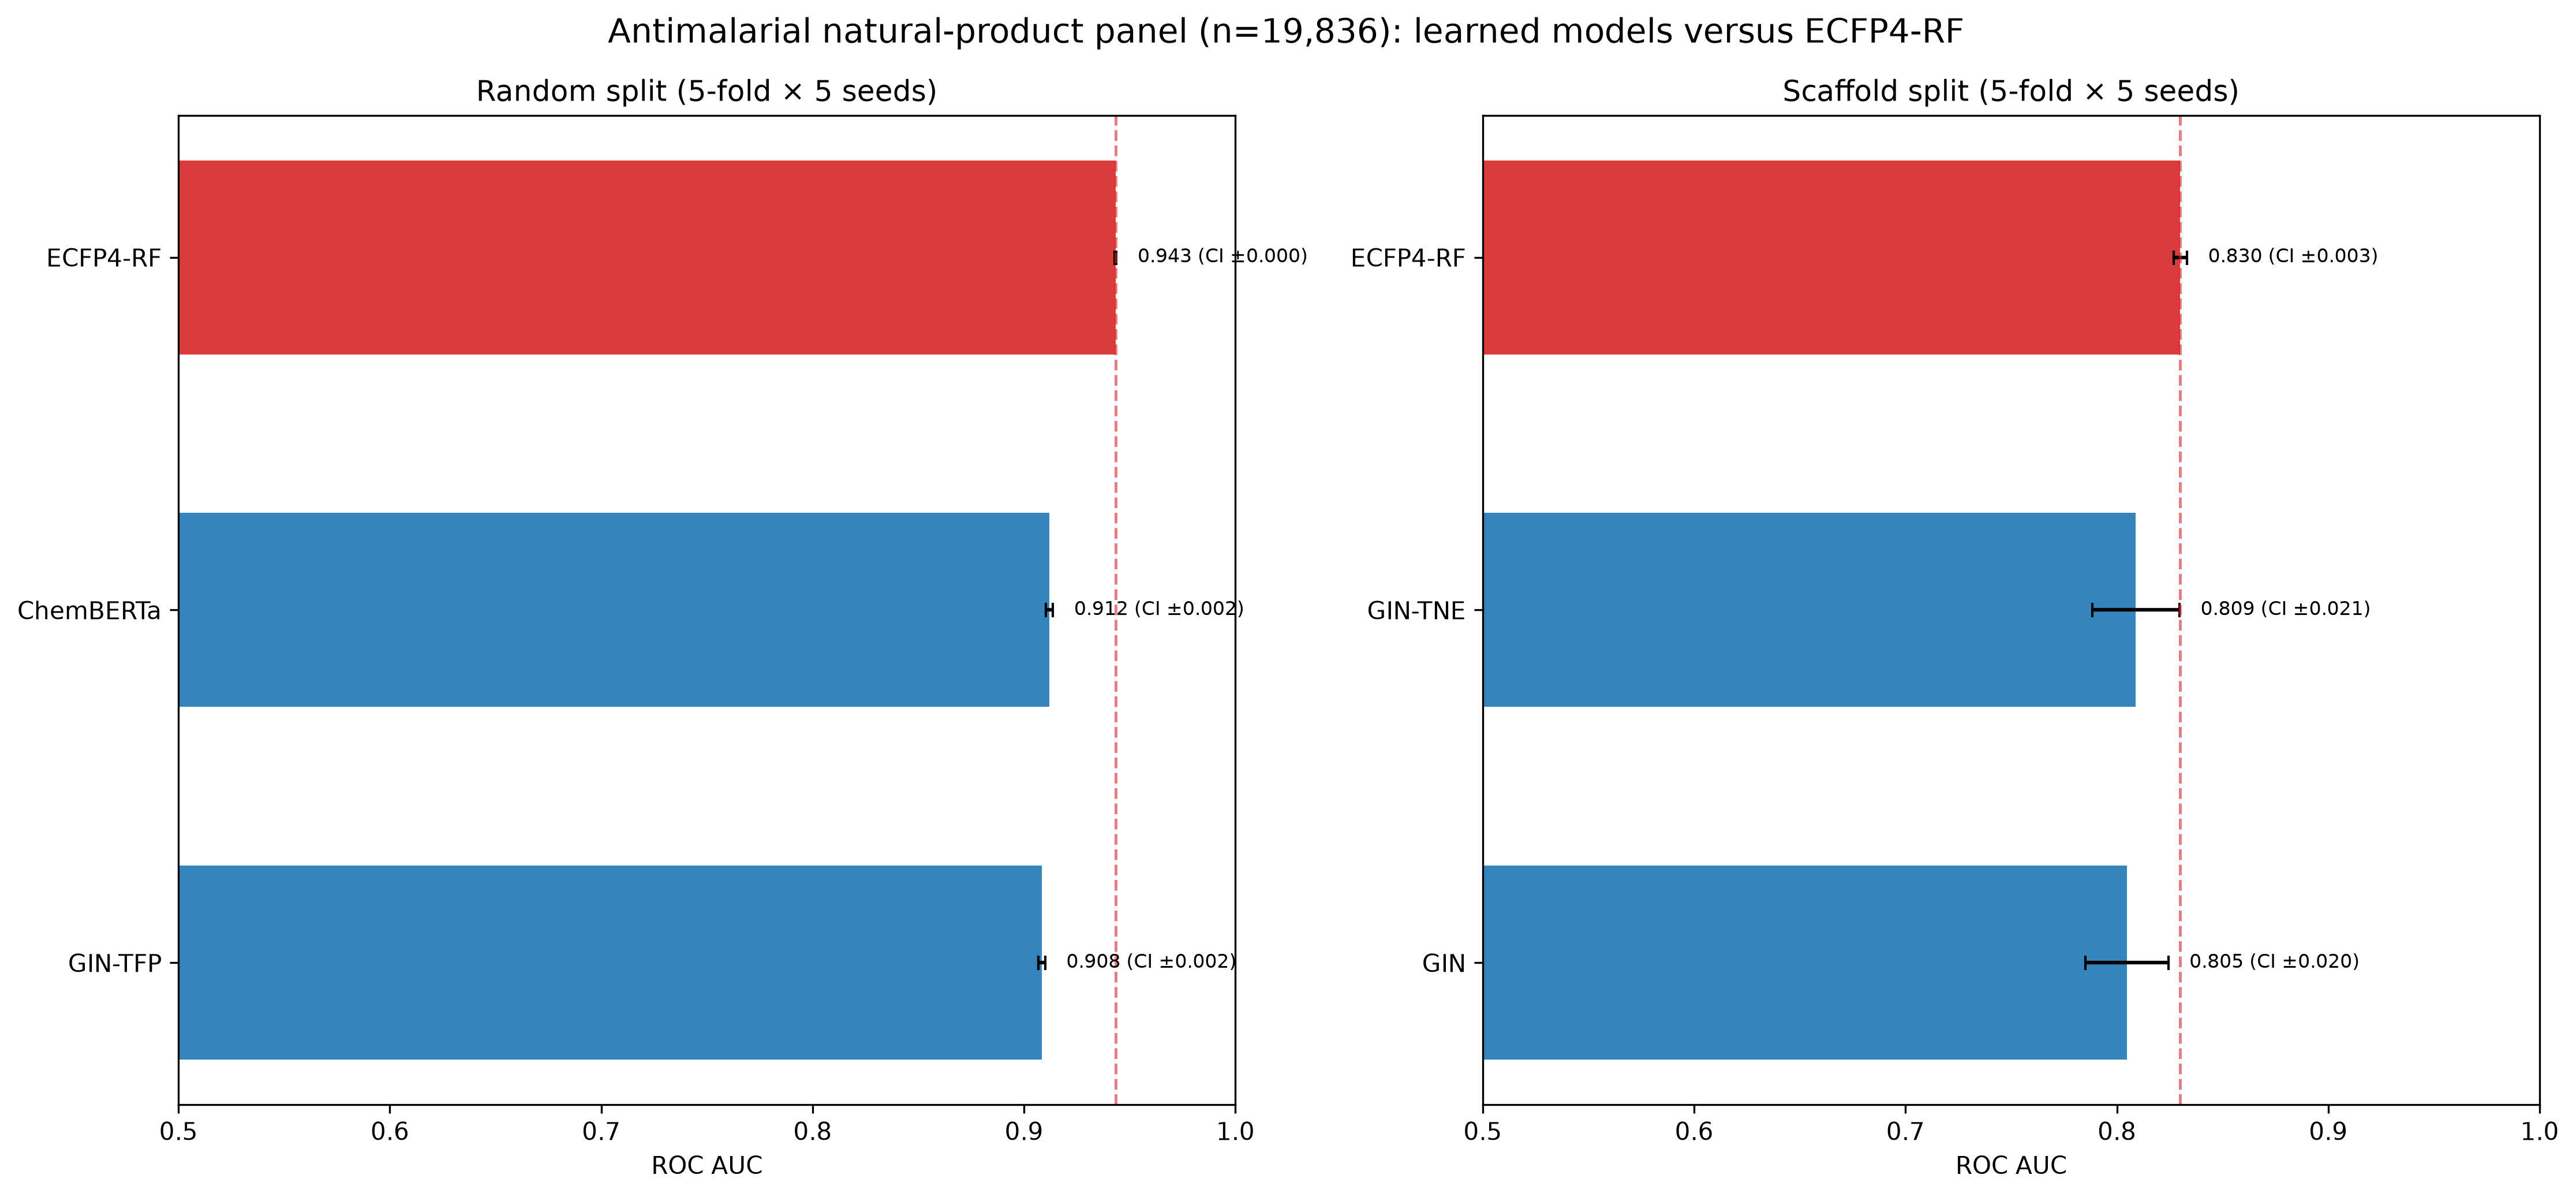
\includegraphics[width=0.98\textwidth]{p5_auc_benchmark.png}
\caption{Mean test ROC AUC (bars) with 95\% confidence intervals, random (left) and scaffold (right) splits, 25 fold--seed replicates per model. The ECFP4--RF baseline (red) is not beaten by any GNN or transformer arm. CIs for the baseline are computed from the five per-seed means; for models, across all 25 fold--seed AUCs.}
\label{fig:benchmark}
\end{figure}

\subsection{H3: persistent-image topological features dominate the predictive signal}

Even when predictive gains are absent, learned fusion weights carry interpretable structure. We compute a \emph{salience} score for each descriptor dimension as the mean absolute weight in the fusion projection layer ($\mathrm{head}_0$) over the 25 replicates. For the TFP fusion (78 dimensions: 33 homology-dimension-0, 25 persistent-image, 20 Betti), the \textbf{persistent-image block (dims 33--58) carries the strongest signal} (mean salience 0.0790) versus homology-0 (0.0485) and Betti (0.0547) blocks; the top five dimensions are persistent-image (42, 43, 52, 53, 54). For the TNE fusion (192 dimensions) the top dimensions are 68, 43, 92, 66, 165, and the top-10\% of dimensions account for 17.3\% of total salience (moderate sparsity).

This result is methodologically important: it shows that topological representations \emph{contribute} signal to activity prediction --- in line with the companion quantum-representation study \citep{temgoua2027quantum} and with the interpretability argument of topological descriptors \citep{tda_review_2025} --- but that this signal, on this panel, does not translate into a ranking advantage over fingerprints. Interpretability and ranking are separable axes; our fusion architectures capture the former without delivering the latter.

\begin{figure}[t]
\centering
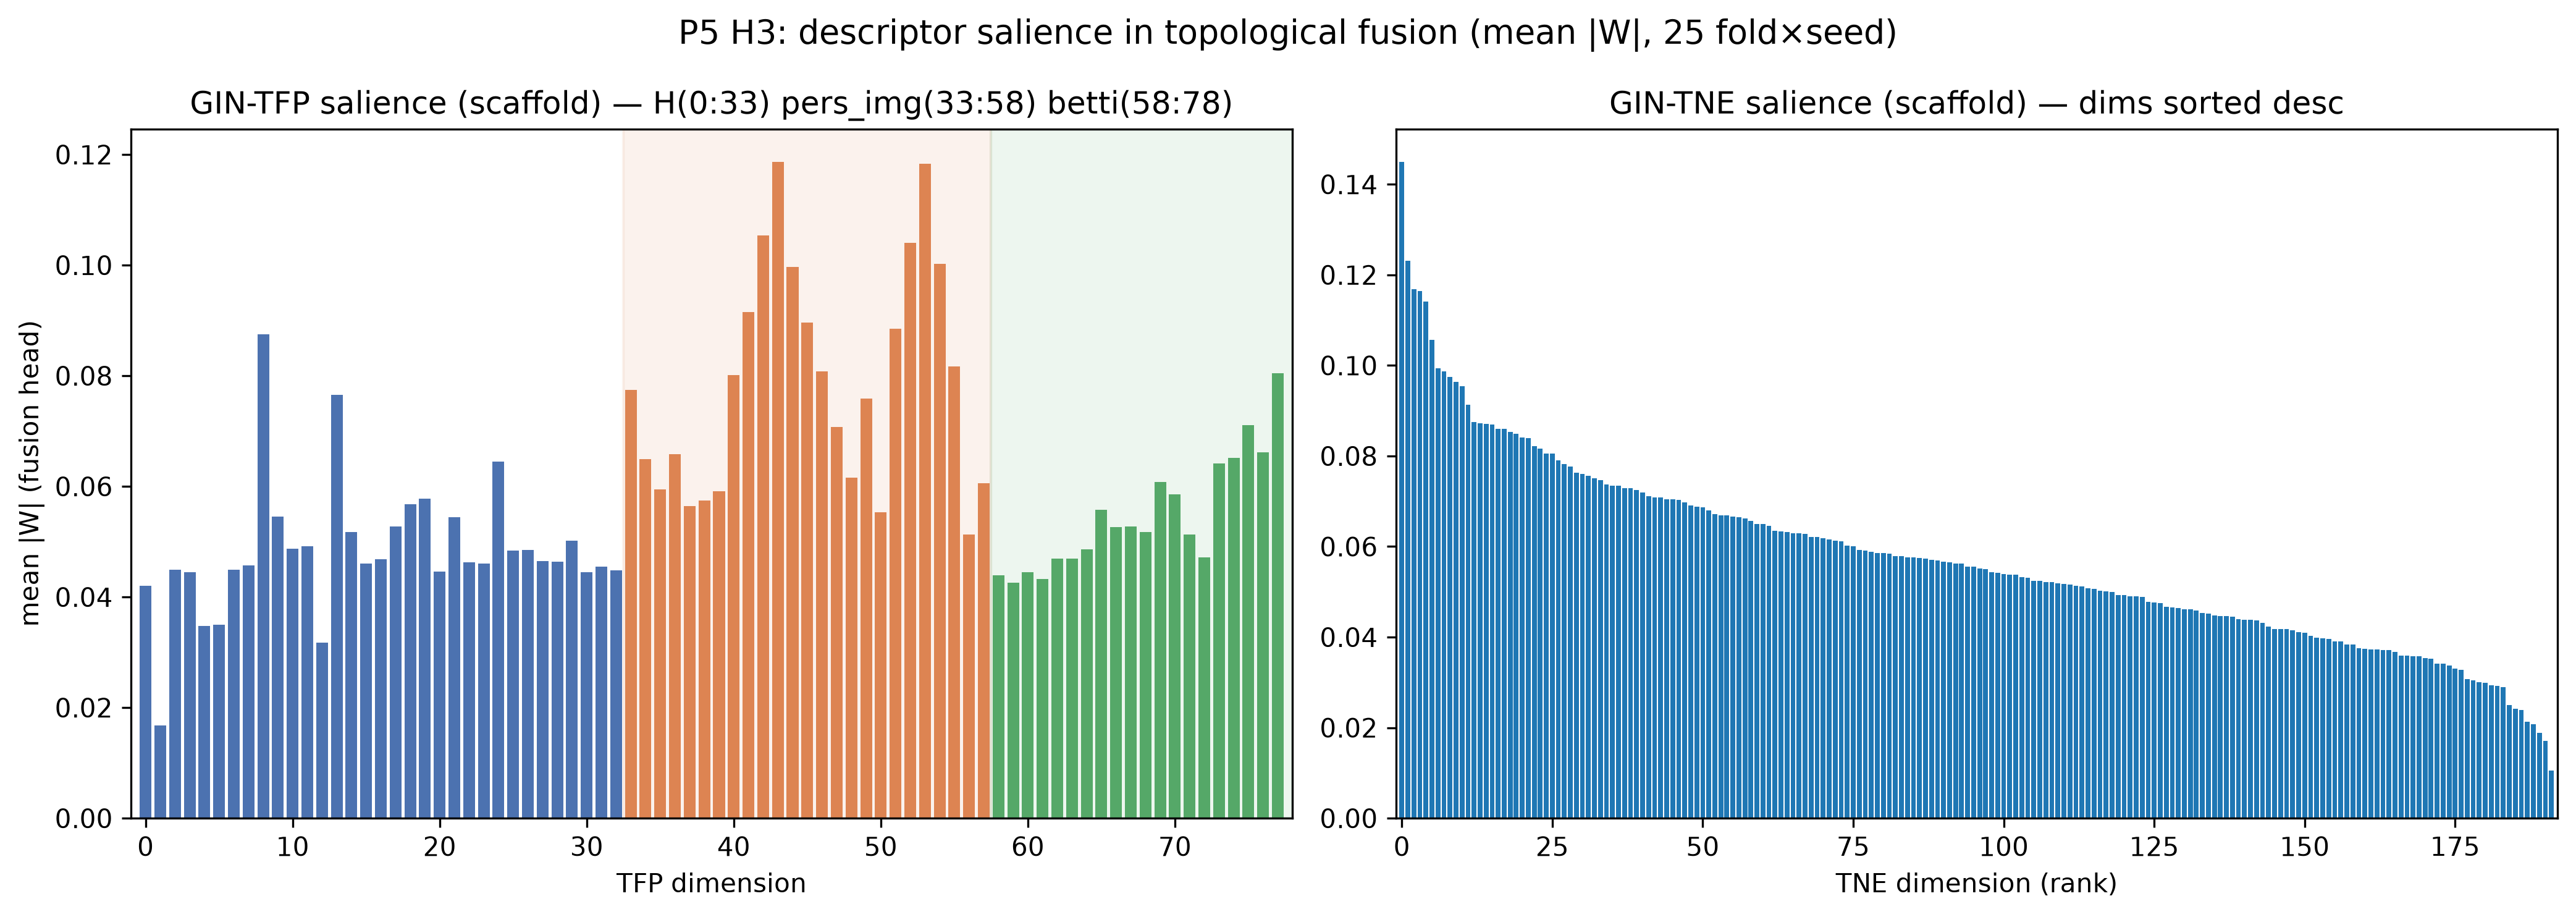
\includegraphics[width=0.98\textwidth]{p5_salience.png}
\caption{Descriptor salience in the topological fusion heads under the scaffold split (mean $|W|$ of the fusion projection layer across 25 fold--seed replicates). Left: TFP (78 dimensions), colored by block --- homology-0 (dims 0--32, blue), persistent-image (dims 33--57, orange), Betti (dims 58--77, green); the persistent-image block carries the strongest signal. Right: TNE (192 dimensions), sorted descending.}
\label{fig:salience}
\end{figure}

\section{Discussion}

\subsection{The verdict is scale-independent and panel-specific}

Our headline result --- \emph{larger, pretrained models do not win on an antimalarial NP panel} --- extends the two most closely related scale-benchmarks \citep{guo_ding_2026,benchmark_pretrained_2025} to a new chemical domain. Three design choices give this negative result evidential force. \emph{First}, the scaffold split is the practically relevant, out-of-distribution protocol for hit-to-lead and library-expansion workflows, and it is the protocol under which the classical advantage is smallest in prior work \citep{guo_ding_2026}; even there, fingerprints lead. \emph{Second}, 25 fold--seed replicates give paired tests adequate power to separate ``no evidence of gain'' from ``significantly worse''. \emph{Third}, the leak audit (H2) shows that the transformer result is not an artifact of weight leakage --- and, symmetrically, that naive implementations \emph{would} have produced inflated, misleading wins. We recommend that transformer benchmark reports state explicitly whether pretrained weights are reset per fold.

\subsection{Why fingerprints hold: representation--task alignment}

The consistent ECFP4 advantage is best explained by representation--task alignment rather than model capacity. ECFP4 encodes local substructure environments; for a collection of structurally related natural products, local SAR is the dominant signal, and tree ensembles exploit it efficiently with few thousand labels \citep{ecfp_2010}. Learned graph representations require more data to recover the same local patterns and generalize to scaffold-held-out series only partially \citep{benchmark_pretrained_2025}. This is consistent with the medicinal-chemistry view that fingerprints plus random forests remain an effective early-stage tool \citep{learning_mol_repr_2020}. The counterpoint that graph models can be made competitive by training them \emph{on} fingerprints is instructive: ECFP-pretrained GNNs improve out-of-distribution performance on homogeneous ADMET tasks but still underperform on heterogeneous endpoints such as binding affinity \citep{ecfp_pretrained_2026}---mirroring the fingerprint-centric explanation, since the pre-training transfers the very substructure knowledge fingerprints encode. Our attribution result (H3) adds a nuance: the topological descriptors are \emph{not} uninformative --- they carry interpretable geometric signal --- but their marginal ranking contribution is small on this panel.

\subsection{Relation to the companion projects}

This benchmark shares its frozen 19,836-molecule panel and fingerprint pipeline with the companion quantum-representation study \citep{temgoua2027quantum}, and both sit inside a programme whose stated goal is the mitigation of antimalarial drug resistance using African natural products: the screening campaign \citep{temgoua2026antimalarial} identified leads validated against resistance mutations by molecular dynamics (PfDHFR N51I/C59R/S108N/I164L; PfCRT K76T) in a companion study \citep{temgoua2027md}. The quantum kernel study reported a similar ``no advantage'' verdict at the kernel level (quantum kernel $\approx$ RBF, $p \ge 0.06$), and identified the persistent-image/topological features as its principal contributors. The present work reaches the same two-part conclusion --- \emph{no ranking advantage, useful attribution} --- from an entirely different model family (GNN/transformer fusion). A companion generative-design study on the same antimalarial program found the analogous structural result for generation: simple random search matches a Pareto-guided MCTS on the scalar reward, whose real value lies in diversity of the Pareto front \citep{temgoua2027mcts}. Taken together, the three studies form a coherent, honest-negative programme: across prediction and generation, and across kernels, graphs, and transformers, representational and algorithmic complexity does not beat simple baselines on scalar objectives on this program; its value is qualitative (attribution, diversity). We believe such honest-negative reporting, with reproducible code and data, is itself a contribution the field currently undervalues \citep{benchmark_pretrained_2025,guo_ding_2026}.

\subsection{Limitations}

Our panel, while curated and clinically motivated, is a single binary-activity collection assembled from screening data; label noise and class imbalance may differ from public benchmarks. The GNN and fusion models use a single-layer architecture and fixed hyperparameters (hidden 128, 50 epochs, patience 10); deeper or better-tuned architectures could close part of the gap, though prior scale-benchmarks find the classical advantage robust to such tuning \citep{guo_ding_2026}. ChemBERTa was fine-tuned with a fixed learning schedule rather than per-task optimization. The salience measure (mean absolute projection weight) is a first-order attribution; more sophisticated methods (e.g., integrated gradients) could refine the H3 conclusion. Finally, the scaffold split is a proxy for novelty; prospective experimental validation remains the ultimate test. A recent structural-frontier analysis reinforces this caveat: a scaffold identifier captures only one notion of chemical unfamiliarity, and splits that reserve the sparsest, physicochemically remote scaffold groups inflate error further on ADMET tasks \citep{scaffold_frontier_2026}; our verdicts should therefore be read as valid for Bemis--Murcko scaffold held-out series, with harder forms of novelty (e.g., distant scaffold-frontier groups) posing an even steeper generalization test.

\section{Methods}

\subsection{Data and panel}

We use the frozen canonical panel of \textbf{19,836 molecules} with binary antimalarial activity labels from the eOS80CH screening collection, curated and deduplicated by canonical SMILES as described in the companion study \citep{temgoua2026antimalarial}. Features: ECFP4 (1024-bit Morgan radius-2), topological fingerprints (TFP, 78 dims: persistent homology-0, persistent images, Betti numbers computed by the companion pipeline), and tensor-network embeddings (TNE, 192 dims). All features are aligned on the canonical panel indices.

\subsection{Splits}

Two protocols, each five-fold, repeated over five seeds (25 fold--seed replicates total). (i) \emph{Random}: stratified five-fold CV. (ii) \emph{Scaffold}: molecules grouped by Bemis--Murcko scaffold before fold assignment, so that no fold shares a scaffold with the training folds. Frozen split indices are released to guarantee cross-project comparability.

\subsection{Models}

\textbf{ECFP4--RF}: scikit-learn RandomForest on ECFP4, the reference baseline. \textbf{GIN}: graph isomorphism network (128 hidden units, mean-pooling readout, single head) trained on molecular graphs (atom/edge features from RDKit). \textbf{GIN--TFP / GIN--TNE}: the same GIN with the topological descriptor vector concatenated at the head ($\mathrm{head}_0 = \mathrm{Linear}(128 + n_{desc} \to 128)$), enabling the salience attribution. \textbf{ChemBERTa}: pretrained SMILES transformer, fine-tuned with cross-entropy and \emph{per-fold weight reset} (see leak audit below). All deep models trained on a single NVIDIA RTX A4000 GPU with AdamW, early stopping on validation AUC (patience 10 of 50 epochs), and best-val checkpoint selection.

\subsection{Leak audit and correction}

Initial ChemBERTa runs loaded the pretrained model once and reused the same instance across all folds, resetting only the optimizer. Because fine-tuning transfers learned weights to the next fold, folds 1--4 inherited previous folds' fine-tuning, inflating test AUCs by up to 0.15 (0.826 honest fold-0 vs. 0.95--0.99 contaminated folds). We fix this by snapshotting the pretrained weights at initialization and reloading them at the start of every fold, making folds independent. All transformer numbers reported here use the corrected protocol; contaminated checkpoints were discarded.

\subsection{Statistics}

Per model, 25 fold--seed AUCs. Model-vs-baseline comparisons use paired $t$-tests on the five per-seed means (each a mean over the five folds). Significance threshold $\alpha = 0.05$; effect sizes reported as mean difference. Salience is aggregated across the 25 replicates as the per-dimension mean absolute projection weight.

\section{Data and code availability}

All scripts, frozen splits, per-fold results, salience data, and figure code are released in the project repository; trained checkpoints and the canonical panel are included. Reproducibility is supported by the frozen split files (random and scaffold), the frozen feature tables, and the pinned environment.

\section{Author contributions}

\section{Conflicts of interest}

\section{Acknowledgements}

\section*{References}
\bibliographystyle{unsrtnat}
\bibliography{Bibliography_P5}

\end{document}
